% work areas are denoted by #####
%
%
%new intro chapter starting 31/05/01

%$Source: /server/cvs/mpiom1/mpi-om/doc/tecdoc_mpiom/Attic/c4.tex,v $\\
%$Revision: 1.1.2.1.4.2.2.2.2.3.2.1 $\\
%$Date: 2006/03/07 14:50:43 $\\
%$Name: mpiom_1_2_0 $\\


%\pagenumbering{arabic}
\thispagestyle{empty}
 
\chapter[Numerical Background]
{\Large{\bf Numerical Background}}
\label{ch:numeric}

Most parts of this chapter are taken from \citet{Marsland:2003} and the {HOPE} model description by \citet{wolff97}.

\section{Ocean Primitive Equations}

The horizontal momentum balance 
for a hydrostatic Boussinesq fluid on a rotating sphere is
\begin{equation}
\label{eqn:mom}
{d{\vec v}_o\over{dt}} + f({\vec k}\times{\vec v}_o) =
- {1\over\rho_w}
\left[
{\vec \nabla}_H(p+\rho_wg\zeta)
\right]
+ {\vec F}_H + {\vec F}_V
\end{equation}
where ${\vec v}_o  = (u_o,v_o)$ is the oceanic horizontal velocity
vector on the orthogonal coordinates,
t is the time,
$f$ is the Coriolis parameter,
$\vec{k}$ is a unit vector normal to the earth's center,
$\rho_w$ is a constant reference density,
${\vec \nabla}_H$ is the horizontal gradient operator,
$p$ is the internal pressure,
g is the acceleration due to gravity
and $\zeta$ is the sea surface elevation.
The total derivative is given by
${d\over{dt}} = {\partial \over{\partial t}} +
\vec{v}_o\cdot {\vec \nabla}_H +
w_o \cdot {\partial \over{\partial z}}$
where $w_o$ is the vertical component of ocean velocity
and ${\partial \over{\partial z}}$ is the vertical partial derivative.
${\vec F}_H$ and ${\vec F}_V$ are parameterizations of horizontal and vertical eddy viscosity, respectively.

Diagnostic treatment of pressure and density
is used to close the momentum balance.
Density $\rho$ is taken to be a function of model pressure,
temperature and salinity according to the
equation of state polynomial defined by
the Joint Panel on Oceanographic Tables and Standards (UNESCO, 1983).
\nocite{unesco83}
Potential temperatures are converted to {\em in situ}
temperatures for the density calculation.
The pressure is calculated using the
hydrostatic equation%(\ref{eqn:hydrostatic})
.
\begin{equation}
\label{eqn:hydrostatic}
{\partial p \over{\partial z}}= -g\rho
\end{equation}

Forward integration of the ocean model surface elevation
is based on a linearized kinematic boundary condition
stating that the time rate of change of surface elevation
is equal to the vertical component of oceanic velocity at
the surface.
\begin{equation}
\label{eqn:zeta1}
{\partial \zeta \over {\partial t}}=
w_o\vert_{z=\zeta}
\end{equation}
The vertical velocity is calculated from the horizontal
velocity field using the incompressibility condition.
\begin{equation}
{\partial w_o \over {\partial z}}= -{\vec\nabla}_{H}\cdot{\vec v_o}
\end{equation}
Integrating over the entire depth gives the
vertical velocity at the sea surface.
\begin{equation}
w_o\vert_{z=\zeta} =
-{\vec\nabla}_H\cdot\int_{-H}^{\zeta}{\vec v_o}\:dz
\end{equation}
Potential temperature $\theta$ and salinity $S$ obey the advection-diffusion equations
\begin{eqnarray}
\label{eqn:tempdiff}
{d{\theta}\over{dt}}
%{\partial \theta \over{\partial t}} 
%+ u_o {\partial \theta \over {\partial x}}
%+ v_o {\partial \theta \over {\partial y}}
%+ w_o {\partial \theta \over {\partial z}}
&=&
%{{\vec \nabla} \cdot {\bf K} \cdot {\vec \nabla} \theta}\\
{\vec \nabla_{H}} \cdot \left( {\bf K} {\vec \nabla_{H}} \theta \right) \\
\label{eqn:saltdiff}
{dS\over{dt}}
%{\partial S\over{\partial t}} 
%+ u_o {\partial S \over {\partial x}}
%+ v_o {\partial S \over {\partial y}}
%+ w_o {\partial S \over {\partial z}}
&=&
%{{\vec \nabla} \cdot {\bf K} \cdot {\vec \nabla} S}
{\vec \nabla_{H}} \cdot \left( {\bf K} {\vec \nabla_{H}} S \right)
\end{eqnarray}
where the tensor {\bf K} is a subgridscale parameterization
of horizontal/iso-neutral and vertical/dianeutral diffusion.

The  surface fields can be relaxed to climatological fields $(\Theta_\star, S_\star)$
by specifying
\begin{eqnarray}
\label{eqn:numeric:relaxation}
D_V{\partial\Theta\over{\partial z}}&=& \lambda (\Theta_\star - \Theta)\\
D_V{\partial S\over{\partial z}}&=& \lambda (S_\star - S)
\end{eqnarray}

Relaxation time constants can be set in the namelist (\ref{tb:using:namelist}).
At lateral boundaries and at the sea floor no flux conditions apply
for heat and salt.
%%%%%%%%%%%%%%%%%%%%%%%%%%%%%%%%%%%%%%%%%%%%%%%%%%%%%%%%%%%%%%%%%%%%%%%%%%%%%%%%%%%%
\section{Ocean Subgridscale Parameterizations}
\label{sec:subgrid}

The coarse horizontal and vertical resolution of OGCMs necessitates the use
of subgridscale parameterizations. The \mbox{MPI-OM} model currently has formulations
for BBL slope transport, 
horizontal and vertical viscosity, 
vertical and isopycnal diffusivity, 
eddy-induced mixing,
and convection, as described below.
With respect to the many parameter choices necessary for inclusion
of subgridscale processes in the \mbox{MPI-OM} model (and OGCMs more generally),
we note the myriad sensitive interactions that such choices have on each other.
Since computational constraints do not currently permit a full spanning
of parameter space
the parameter choices used in the present version of \mbox{MPI-OM}
are a necessary blend of those gained via past experience with the HOPE model,
those available from the bandwidth of literature values,
and those that were tuned (in a sometimes {\em ad hoc} manner
traditionally referred to as the art of numerical modeling)
to give iteratively improved results as part of the model development process.
The latter is relevant to, for example, our choices of friction, diffusion, convection
and wind mixing parameters.

\subsection{Slope Convection}
\label{sec:bbl}
The thermohaline circulation of the world's ocean is maintained by the sinking of dense
water masses in high latitudes. In most cases these water masses form in marginal
seas or on shelves and slide down the continental slopes. One particular
phenomenon is the `overflow', where dense near-bottom waters cross sills between
ocean basins (e.g.\ Price and Baringer, 1994).\nocite{price94}
This process is not well resolved
in coarse-resolution z-coordinate ocean models owing to a lack of a BBL.
In such models the dense water passing over a sill is advected
horizontally and placed above lighter water. The resulting convection (parameterized
as strong mixing or intensified diffusion) leads to an overestimation of the
mixing between the overflow and the ambient water.
To overcome this problem \citet{beckmann97} developed a BBL
parameterization where the horizontal flow is redirected as if it flowed along
the bottom. 
This approach to the BBL problem can be avoided 
by the use of $\sigma$-coordinate models (e.g.\ Ezer and Mellor, 1997),\nocite{ezer97}
which are been compared to both isopycnal and z-coordinate models in 
the Dynamics of Overflow, Mixing and Entrainment (DOME) Project. 
Advantages and disadvantages of the various vertical coordinate systems are discussed 
by the \citet{dynamo97} or on the DOME webpage 
(www.rsmas.miami.edu/personal/tamay/DOME/dome.html).

In the HOPE model a relatively simple slope convection scheme
was introduced by \citet{legutke2001}.
In the Legutke and Maier-Reimer scheme the slope convection
was considered to be a directional diffusive transport whereby
an exchange of tracer occurs between the bottom cells
of two adjacent horizontally discretised water columns.
The BBL scheme newly introduced into \mbox{MPI-OM}
is schematically represented in Fig.~\ref{fig:bbl}
which shows the BBL transport Tr$_{\mathit BBL}$ from a source cell to a target cell.
The implementation is similar to that of \citet{beckmann97}
with two notable exceptions.
Firstly, the BBL thickness $H_{\mathit{BBL}}$
may be less than the model layer thickness $\Delta z_s$ of the source cell.
That is,
\begin{equation}
\label{eqn:bbl1}
H_{\mathit{BBL}} = \min \left( \Delta z_s, \mathit{BBL}_{\mathit{max}} \right)
\end{equation}
where BBL$_{\mathit{max}}$ is a prescribed maximum thickness.
The motivation is to limit the BBL transport
in coarse vertical resolution ocean models where
the deeper grid cells can be of order 1~km thickness.
Secondly, as suggested by \citet{campin99}
the BBL transport is redirected to a level of neutral buoyancy
rather than to the bottom cell of a horizontally adjacent water column.
For a source cell having density $\rho_s$ at model level k$_s$,
the target cell level k$_t$ is chosen by the following condition.
\begin{equation}
\label{eqn:bbl2}
k_t=\left\{\begin{array}{lllll}
k_{\rho} & \mathit{if} & \rho_t \le \rho_s & 
{\mathit{and}} & \rho_{t+1} > \rho_s \\
k_{\mathit{bot}} & \mathit{if} & \rho_{\mathit{bot}} \le \rho_s &&
\end{array}
\right.
\end{equation}
Here, the subscript $\mathit{bot}$ denotes the deepest wet model layer in a target column.
The neutral buoyancy approach is particularly useful in regions
where coarse horizontal resolution does not allow
for a gradual descent on a staircase-like slope.
The resultant BBL transport is given by
\begin{equation}
\label{eqn:bbl3}
Tr_{\mathit BBL} = u_s \Delta x,y H_{\mathit{BBL}}
\end{equation}
where $u_s$ represents the meridional (parallel) velocity in the model level k$_s$,
and $\Delta x,y$ represents the parallel (meridional) source cell width.
The remaining advective transport is given by
\begin{equation}
\label{eqn:bbl4}
{\mathit{Tr}} = u_s \Delta x,y (\Delta z_s - H_{\mathit{BBL}})
\end{equation}
and is purely horizontal.
Although not used in this study,
\mbox{MPI-OM} also includes
an improved version of the BBL scheme where $H_{\mathit{BBL}}$ is calculated locally
depending on the stratification and friction velocity using the formulation of \citet{killworth99}.


\begin{figure}[!tb]%\psdraft
\centerline{\hbox{\fbox{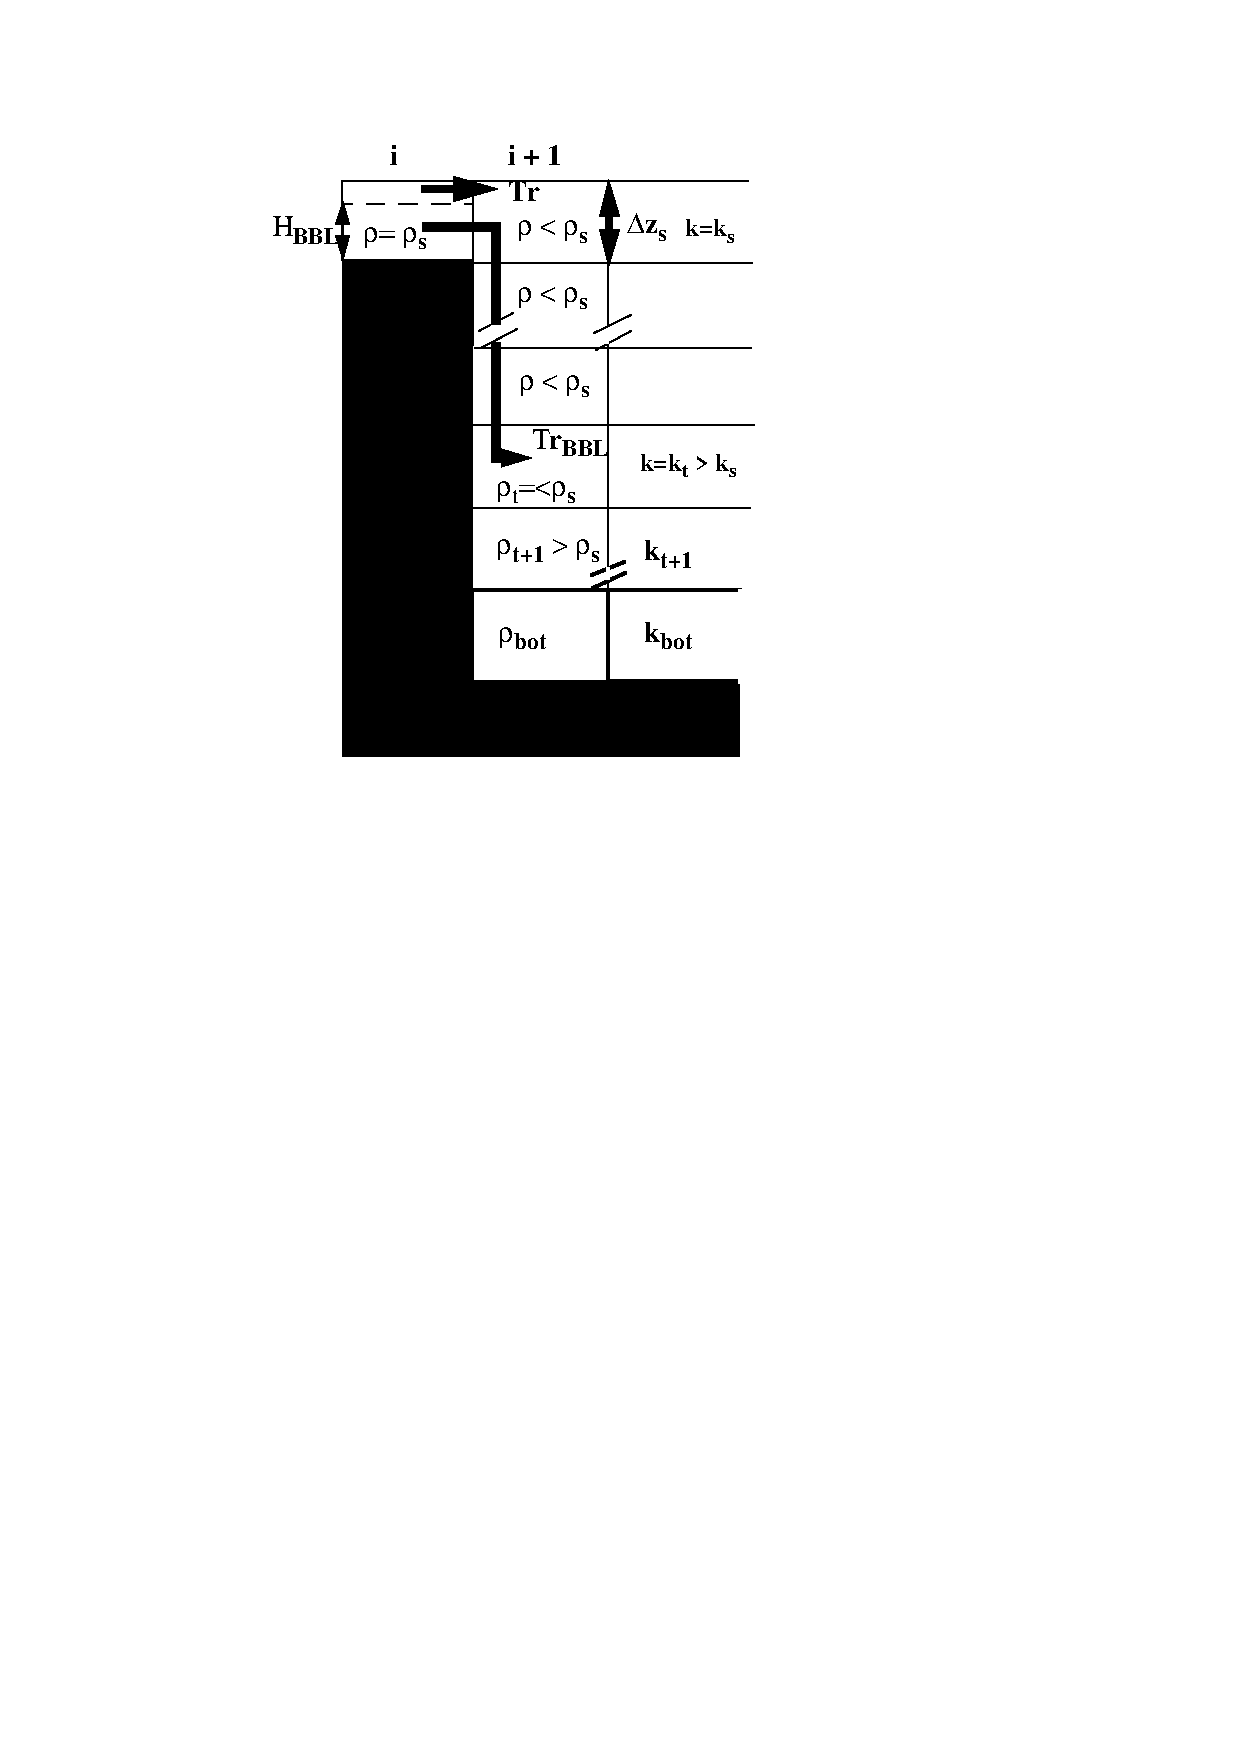
\includegraphics[width=6.cm,angle=0,clip]{bblschem}}}}
\caption{Schematic diagram of the bottom boundary layer advective transport to neutral density level.
Model levels are indicated by k where
k$_s$ and k$_t$ indicate the levels of the source and target cells respectively.
The grid index i refers to either meridional or parallel directions in the curvilinear 
horizontal discretization.
For additional details refer to the text.
}
\label{fig:bbl}
\end{figure}

\subsection{Eddy Viscosity}


The horizontal and vertical eddy viscosity are treated separately.
Horizontal eddy viscosity ${\vec F}_H$ is parameterized 
using a scale-dependent biharmonic formulation
\begin{equation}
\label{eqn:momvisc}
{\vec F}_H =
%- {\vec \nabla_{H}} B_H {\vec\nabla}^3_{H}{\vec v_o}
%- {\vec \nabla_{H}} {\vec B}_H {\vec\nabla_H} \Delta_H {\vec v_o}
- {\vec \nabla_{H}} \cdot \left( B_H {\vec\nabla_H} \Delta_H {\vec v_o} \right)
\end{equation}
where $B_H$ is a coefficient proportional to the fourth power
of the grid spacing.
 
Vertical eddy viscosity ${\vec F}_V$ is parameterized as
\begin{equation}
\label{eqn:vedd}
{\vec F}_V =
{\partial \over {\partial z}}
\left(A_V{\partial \over {\partial z}}{\vec v}_o \right).
\end{equation}
The eddy coefficient $A_V$ is partially relaxed to the value at the previous time step
by use of a time filter to avoid 2$\Delta t$ oscillation.
Using $n$ and $\Lambda_V$ to denote the time increment and relaxation coefficient gives:
\begin{equation}
\label{eqn:vedd2}
{A_V}^n =
\left(1 - \Lambda_V\right){A_V}^{n-1} + \Lambda_V\left(A_{\mathit{VO}}\left(1 + C_{\mathit{RA}}R_i\right)^{-2}
+ A_w + A_b\right).
\end{equation}
The time linear relaxation coefficient $\Lambda_V$ is set to 0.6
in accordance with past experience.
Following Pacanowski and Philander (PP; 1981)\nocite{pacanowski81}
the Richardson number $R_i$ dependent mixing term includes constant coefficients $A_{\mathit{VO}}$ and $C_{\mathit{RA}}$. A small constant background viscosity representing mixing by internal wave breaking is denoted by $A_b$.
The PP scheme in its classical form underestimates turbulent mixing close to the surface. Therefore an additional parameterization for the wind induced stirring $A_w$ is included.  
The near surface wind mixing is proportional to the cube of the local ten meter wind speed $V_{10m}$,
and is reduced in proportion to the fractional sea ice cover $I$.
It decays exponentially with depth and depends on the local static stability $\delta_z \rho$.

\begin{eqnarray}
\label{eqn:awmix}
{A_w(1)}&=&{(1-I) W_T  V_{10m}^3}\\
{A_w(k)}&=&{A_w(k-1) {{\lambda \over{\Delta z}} \over{{\lambda \over{\Delta z}}+ \delta_z \rho}} e^{\Delta z \over{z_0}}  }
\end{eqnarray}
where k=2,3,...,$k_{bot}$ is the vertical level and $\Delta z$ is the level thickness; 
$\lambda$, $z_0$, and $W_T$ are adjustable parameters which were tuned for optimal mixed layer depths.

Tracer diffusion in Eqns~\ref{eqn:tempdiff} and \ref{eqn:saltdiff} 
is represented in two optional ways. The diffusion tensor {\bf K} 
can be chosen either to represent: 
a) standard horizontal/vertical diffusion
\begin{equation}
\label{eqn:khor}
{\bf K} = { D_H \left[ \matrix{1 & 0 & 0 \cr
                     0 & 1 & 0 \cr
                     0 & 0 & \epsilon}\right]}
\end{equation}
with $\epsilon={D_V \over{D_H}}$ ; or
b) isoneutral/dianeutral diffusion

\begin{equation}
\label{eqn:kiso}
{\bf K} = { D_H \left[ \matrix{1 & 0 & S_x \cr
                                0 & 1 & S_y \cr
                   S_x & S_y & \epsilon + S_{\mathit{dif}}^2}\right]}
\end{equation}

with $\epsilon={D_V \over{D_H}}$
and $S_{\mathit{dif}} = (S_x, S_y, 0 )
       = ( {-\delta_x \rho \over{\delta_z \rho}}
       ,   {-\delta_y \rho \over{\delta_z \rho}} 
       ,0 )$.\\ 
The transformation follows \citet{redi82}  with the small slope approximation by 
\citet{gent95}. 
The scheme is numerically implemented following \citet{griffies98b}.
%All the experiments presented in this article utilise 
%isoneutral/dianeutral diffusion.

The effect of tracer mixing by advection with the unresolved mesoscale eddies
is parameterized after Gent et al. (1995).  
 
The vertical eddy diffusivity coefficient $D_V$ is treated similarly to 
Eqn~\ref{eqn:vedd2},
except for the cubic dependence on the shear instability-dependent (Richardson number) term:
\begin{equation}
\label{eqn:hedd}
{D_V}^n =
\left(1 - \Lambda_D\right){D_V}^{n-1} + \Lambda_D\left(D_{\mathit{VO}}\left(1 + C_{RD}R_i\right)^{-3}
+ D_w + D_b\right).
\end{equation}
As with the vertical viscosity,
$D_{\mathit{VO}}$, $C_{RD}$ and the small background term $D_b$ are constant.
The wind-induced term $D_w$ is treated in the same manner as for viscosity.

There are several choices for parameterization of convection currently available in the \mbox{MPI-OM} model.
For details please see \ref{ch:timestepping:octher}

%Convective adjustment follows \citet{bryan69}. 
%Traditionally this technique involved the full mixing of vertically adjacent grid cells 
%in the presence of static instability.
%The \mbox{MPI-OM} formulation is similar but only mixes the upper grid cell with an equivalent thickness
%of the lower grid cell.
%This approach aims to increase the penetrative depth of convection.
%Alternatively \mbox{MPI-OM} allows for the use of a much more physically based parameterization based on the
%penetrative plume convection scheme of \citet{paluszkiewicz97}.
%Plume convection was found to significantly improve the deep water characteristics and
%the simulation of Southern Ocean sea ice in the {HOPE} model \citep{kim2001}.
%However, the penetrative plume convection scheme is computationally quite expensive and is not used
%in the simulations described in this paper.
%The third scheme, and also the one used in this study, is the parameterization of convection
%by greatly enhanced vertical diffusion in the presence of static instability
%(e.g.\ Marotzke, 1991; Klinger at al., 1996). \nocite{marotzke91,klinger96}
%Such an approach avoids the excessive intermediate mixing associated with the traditional adjustment scheme
%by introducing a timescale associated with the choice of (constant) convective-diffusion coefficient.



%%%%%%%%%%%%%%%%%%%%%%%%%%%%%%%%%%%%%%%%%%%%%%%%%%%%%%%%%%%%%%%%%%%%%%%%%%%%%%%
\section{Model Grid}
\label{ch:numeric:grid}




% horizontal discretization
Horizontal discretization of the \mbox{MPI-OM} model is on a staggered Arakawa C-grid \citep{arakawa77}.
The reference grid is shown in figure \ref{fig:numeric:grid:horizontal}.
It consists of prism-shaped finite volumes with the edges aligned with coordinates. 
Vertical discretization is on a so called `z-coordinate' system 
(differentiating from pressure or density coordinate systems).

\subsection{Horizontal discretization}
\label{ch:numeric:grid:horizontal}


\begin{figure}[!!!h]
\centerline{\hbox{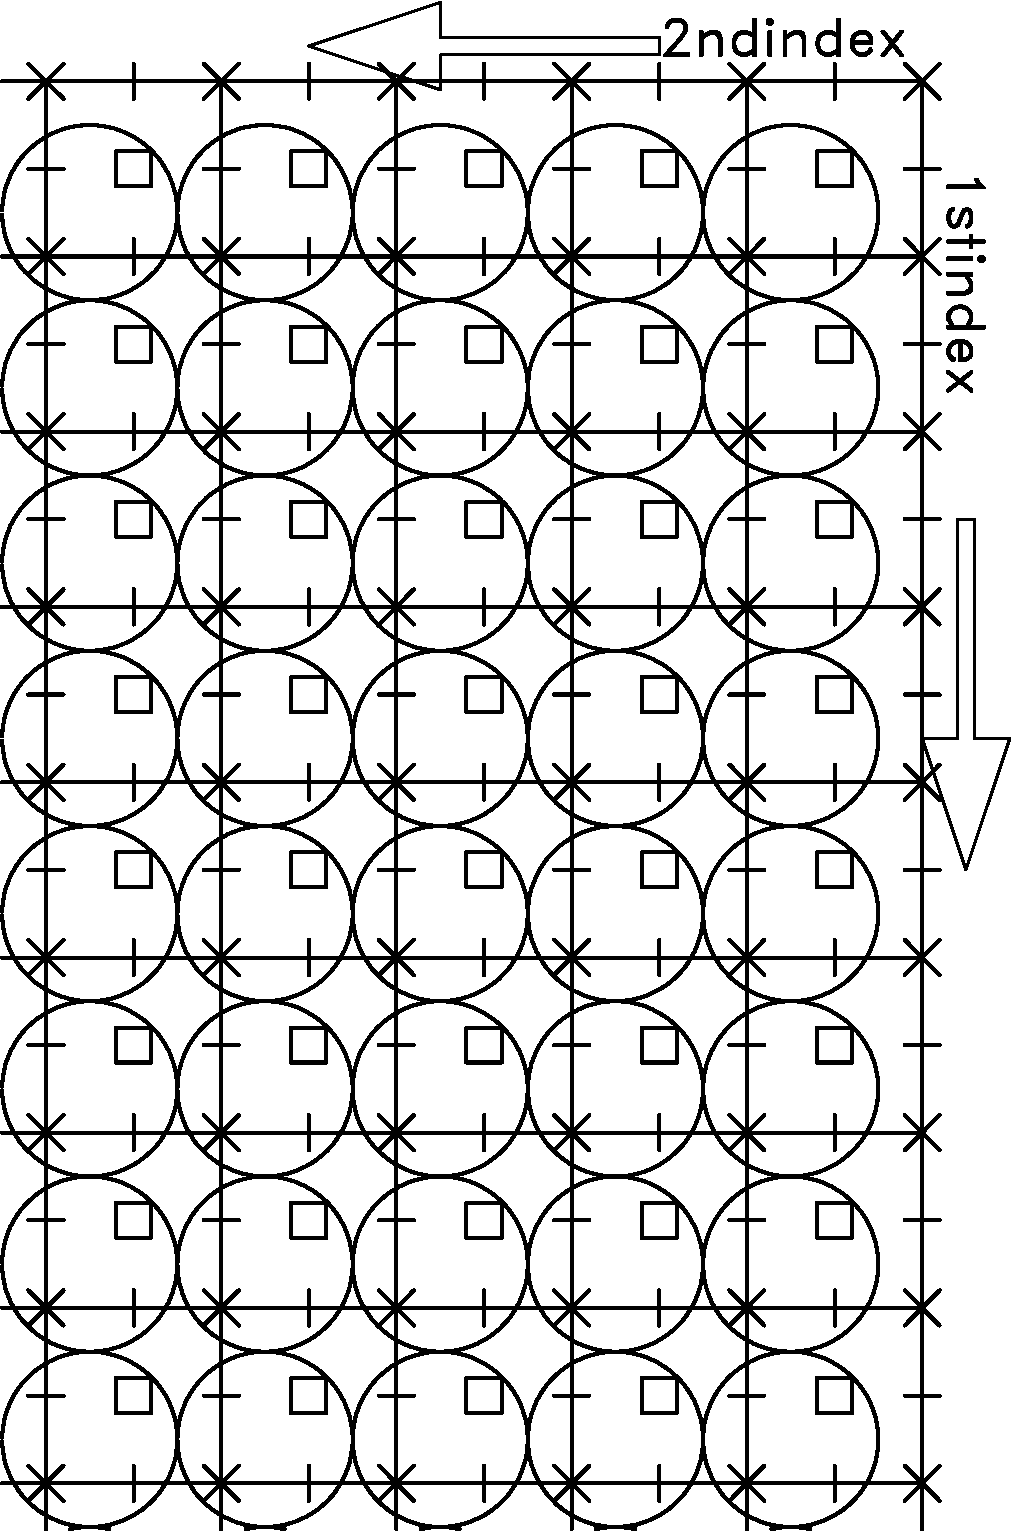
\includegraphics[width=10.0cm,angle=90,clip]{cgricon_new}}}
\mycaption{Layout of the Arakawa C--grid. Boxes denote scalar points, slashes vector points (u in i-direction and v in j-direction) and stars 
the points where the stream function $\psi$ is defined.}
\label{fig:numeric:grid:horizontal}
\end{figure}


Variables defined on vector points are :
\begin{itemize}
\item{horizontal velocities $(u,v)$} 
\item{wind stress $\underline\tau=(\tau^\phi ,\tau^\lambda)$}  
\item{coefficients of vertical viscosity} 
\end{itemize}
Variables defined on scalar points are :
\begin{itemize}
\item{potential temperature $\Theta$} 
\item{salinity $S$} 
\item{density $\rho$} 
\item{pressure $p$} 
\item{vertical velocity $w$}  
\item{coefficients of vertical diffusivity} 
\item{sea surface elevation $\zeta$} 
\item{heat-- and freshwater fluxes across the air sea interface} 
\end{itemize}
Diagnostic stream functions are defined in the $\psi$ points of the grid.

Multiple grid-refinements on an orthogonal grid are possible, i.e.\ MPI-OM calculates a grid using
two vectors, one containing information on longitudes
and one on latitudes. A high resolution in a specified region may cause very ``slim'' grid cells
elsewhere. 

Indexing is done as follows:

West -- East : $\mbox{\tt I} = 1,\ldots,\mbox{\tt IE}$,\\
North -- South : $\mbox{\tt J} = 1,\ldots,\mbox{\tt JE}$,\\
Sea surface -- Bottom : $\mbox{\tt K} = 1,\ldots,\mbox{\tt KE}$

The points with west--east indices 1 and 2
correspond to points with indices {\tt IE-1} and {\tt IE}, respectively,
when periodic boundaries are chosen.


The spherical geometry of the earth is taken into
account by storing all grid distances
$\Delta x(\lambda,\phi)$ and $ \Delta y(\lambda,\phi)$ on arrays, which are then used in the discretization
formulas.

\subsection{Vertical discretization}
\label{ver}

The vertical discretization is the same as used in the {HOPE} model \citep{wolff97},
which includes partial vertical grid cells, i.e.\ at each point in the horizontal grid
the deepest wet cell has a uniform thickness that is adjusted to resolve the discretised bathymetry.
The surface layer thickness is also adjusted to account for the sea surface elevation and 
the sea ice/snow draft where appropriate.

%\vspace{2.0cm}
\unitlength1.0cm
%
\newsavebox{\vecscal}
\savebox{\vecscal}(0,0)[l]{
% plus fuer zeta  2mm
\put(0.4,0.5){\line(1,0){0.2}}
\put(0.5,0.4){\line(0,1){0.2}}
% x fuer vektorpunkte 2mm
\put(1.5,0.5){\circle*{0.2}}
}
%
\newsavebox{\wdot}
\savebox{\wdot}(0,0)[l]{
\put(0.5,0.5){\circle{0.2}}
% abgrenzung i=const
}

\begin{figure}[h]
\begin{picture}(15,9)
% sea surface line at y=9cm
\thinlines
\put(0.,9){\line(1,0){14}}\put(14.3,9.0){\makebox(1,0)[l]{$w_1(z=0)$}}
\put(0.,7){\line(1,0){14}}\put(14.3,7.0){\makebox(1,0)[l]{$w_2, A_{V2}, D_{V2}$}}
\put(0.,3){\line(1,0){14}}\put(14.3,3.0){\makebox(1,0)[l]{$w_k, A_{Vk}, D_{Vk}$}}
\put(0.,0){\line(1,0){14}}\put(14.3,0.0){\makebox(1,0)[l]{$w_{k+1}$}}
\put(14.3,8.0){\makebox(1,0)[l]{$p_1, {\bf v}_1$}}
\put(14.3,5.0){\makebox(1,0)[l]{$p_2, {\bf v}_2$}}
\put(14.3,1.5){\makebox(1,0)[l]{$p_k, {\bf v}_k$}}
%
% scalar vector lines
%
\multiput(6.0,7.75)(2.0,0.0){4}{\usebox{\vecscal}}
\multiput(6.0,4.75)(2.0,0.0){4}{\usebox{\vecscal}}
\multiput(6.0,1.25)(2.0,0.0){4}{\usebox{\vecscal}}
\multiput(6.0,8.75)(2.0,0.0){4}{\usebox{\wdot}}
\multiput(6.0,6.75)(2.0,0.0){4}{\usebox{\wdot}}
\multiput(6.0,2.75)(2.0,0.0){4}{\usebox{\wdot}}
\multiput(6.0,-0.25)(2.0,0.0){4}{\usebox{\wdot}}
%
% topography
%
\thicklines
\put(5.,1.){\line(1,0){4.5}}
\put(9.5,1.){\line(0,1){1.5}}
\put(9.5,2.5){\line(1,0){2}}
\put(11.5,2.5){\line(0,1){1}}
\put(11.5,3.5){\line(1,0){2}}
\put(13.5,3.5){\line(0,1){5.5}}
%
% w-vectors
%
\put(6.5,0.){\vector(0,1){1.0}}
\put(8.5,0.){\vector(0,1){1.0}}
\put(10.5,3.){\vector(0,-1){.5}}
\put(12.5,3.){\vector(0,1){.5}}
%
% distances
%
\put(1.5,8.4){\vector(0,1){0.6}}
\put(1.3,8.0){\makebox(1,0)[l]{$\Delta z_{w1}$}}
\put(1.5,7.6){\vector(0,-1){0.6}}
%
\put(1.3,5.4){\vector(0,1){1.6}}
\put(1.1,5.0){\makebox(1,0)[l]{$\Delta z_{w2}$}}
\put(1.3,4.6){\vector(0,-1){1.6}}
%
\put(1.1,1.9){\vector(0,1){1.1}}
\put(0.9,1.5){\makebox(1,0)[l]{$\Delta z_{wk}$}}
\put(1.1,1.1){\vector(0,-1){1.1}}
%
% distances u-points
%
\put(3.7,8.8){\vector(0,1){0.2}}
\put(3.7,8.5){\makebox(1,0)[l]{$\Delta z_{u1}$}}
\put(3.7,8.2){\vector(0,-1){0.2}}
%
\put(3.5,6.9){\vector(0,1){1.1}}
\put(3.3,6.5){\makebox(1,0)[l]{$\Delta z_{u2}$}}
\put(3.5,6.1){\vector(0,-1){1.1}}
%
\put(3.3,2.8){\vector(0,1){2.2}}
\put(3.1,2.4){\makebox(1,0)[l]{$\Delta z_{uk}$}}
\put(3.3,2.0){\vector(0,-1){0.6}}
%
\put(5.3,0.4){\vector(1,1){0.6}}
\put(1.8,0.5){\makebox(1,0)[l]{Model topography}}
% actual layer thicknesses
\put(7.8,6.0){\vector(0,1){1.0}}
\put(7.6,5.6){\makebox(1,0)[l]{$d_{u2}$}}
\put(7.8,5.2){\vector(0,-1){2.2}}
%
\put(7.8,2.5){\vector(0,1){0.5}}
\put(7.6,2.1){\makebox(1,0)[l]{$d_{uk}$}}
\put(7.8,1.7){\vector(0,-1){0.7}}
%
\put(9.8,6.0){\vector(0,1){1.0}}
\put(9.6,5.6){\makebox(1,0)[l]{$d_{u2}$}}
\put(9.8,5.2){\vector(0,-1){2.7}}
\end{picture}
\caption{\label{fig:numeric:grid:vertical} Vertical structure of model grid }
\end{figure}


The choice of depth values at vector points, and thus the assignment
of layer thicknesses, is free. The vertical velocity component is then
computed  as indicated in fig.\ \ref{fig:numeric:grid:horizontal}.
Model arrays are defined as follows:

\label{depp}
\begin{description}
\item {Array({\sl dimensions})} : description
\item {\tt DZW(KE)} : Vertical distance between two
vertical velocity points (layer thickness). The layer thicknesses
are set in the main program via {\tt DATA DZW / \ldots /} and may be
changed by the user. All other vertical distances are computed from this
array.
\begin{eqnarray*}
  \mbox{\tt DZW(K)} = \Delta z_{wk}\qquad k=1,\ldots,\mbox{\tt KE}
\end{eqnarray*}
%
\item{\tt TIESTW(KE+1)} : Actual depth of $w-$ levels
 ({\tt TIESTW(1)}=0)
\begin{eqnarray*}
 \mbox{\tt TIESTW(K)} = \sum_{l=2}^k \Delta z_{wl-1}\qquad k=2,\ldots,\mbox{\tt KE}
\end{eqnarray*}
\item{\tt TIESTU(KE+1)} : Actual depth of vector/scalar levels
(depend only on $k$)
\begin{eqnarray*}
 \mbox{\tt TIESTU(K)} = {\tt 0.5 * (TIESTW(K+1)-TIESTW(K))}\qquad
 k=1,\ldots,\mbox{\tt KE}
\end{eqnarray*}
\item{\tt DZ(KE)} : Vertical distance between two vector/scalar
 points (for K=1 this is half of the first layer thickness)
\begin{eqnarray*}
 \mbox{\tt DZ(K)} = \Delta z_{uk}\qquad k=1,\ldots,\mbox{\tt KE}
\end{eqnarray*}
%
\end{description}

After a  topography dataset has been supplied on the user specified
grid (at the positions of vector points) MPI-OM recalculates the actual depth of scalar points as
the maximum depth of the four surrounding vector points.
Having done this, local layer thicknesses are computed  taking into account
the adjustment of near bottom vertical velocity points (see fig.\ \ref{fig:numeric:grid:vertical}).

The layer thicknesses are stored on arrays {\tt DDUE, DDUO} and {\tt DDPO}
\begin{description}
\item {${\tt DDU}_{E/O}{\tt (IE,JE,KE)}$} : Layer thicknesses at vector points
\item {${\tt DDPO}{\tt (IE,JE,KE)}$} : Layer thicknesses at scalar points
\end{description}
where E/O indicate the vector points in u and v direction.


\subsection{Curvilinear Coordinate System}
\label{ch:numeric:curvilinear}


\begin{figure}[!tb]%\psdraft
\centerline{\hbox{\includegraphics[height=14.cm,angle=-90,clip]{grob_grid}}}
\caption{Standard \mbox{MPI-OM} orthogonal curvilinear grid for global climate study applications at MPIfM.}
\label{fig:numeric:antagrid}
\end{figure}

% curvilinear coord system
The \mbox{MPI-OM} model uses a bipolar orthogonal spherical coordinate system.
If the poles are antipodes (diametrically opposed) then the coordinate system
is reduced to a rotated spherical grid.
Otherwise, orthogonal meridians and parallels are constructed
according to the choice of zonal and meridional resolution and are used to define the spatial mesh.
Although it may be desirable to maintain `quadrature' of the grid
(i.e.\ within each grid cell the local zonal and meridional grid distances are equal),
it is by no means a necessary condition.
Two advantages can be achieved by assignment of a radius to the poles.
Firstly, land points can be removed from the computational matrix.
Secondly, by choosing non-equal pole radii horizontal resolution can be
concentrated about the pole of smaller radius for regional studies.
Implementation of the curvilinear grid is relatively straightforward
but does require 
some additional computational expense.
In terms of memory many additional arrays must be added for storage of all terms
related to horizontal metrics between both scalar and vector neighboring pairs.
The processing time is therefore extended for all operations including horizontal metrics
that could otherwise be factored on a regular grid.
This condition is omnipresent throughout the model code with the exception of purely vertical
operations such as convection.

The standard MPIfM horizontal ocean grid used for climate studies has traditionally been at a spatial resolution
approximating spectral truncation T42 with additional equatorial meridional grid refinement
(e.g.\ HOPE, Legutke and Voss, 1999; OPYC, Roeckner at al., 1999). \nocite{legutke99,roeckner99}
With the 2005 IPCC experiments this has changed to the GROB15 grid with a formal
resolution of 1.5~\degs. In this setup,
one pole is located over Greenland and the other over Antarctica.
The horizontal resolution gradually varies between 10 km in the Arctic
and about 170 km in the Tropics. This arrangement gives highest resolution in the 
main sinking regions associated with the thermohaline circulation (THC).
It has 40 vertical levels with level
thickness increasing with depth. Eight layers are within the upper 90 m
and 20 are within the upper 600m. Also common is the GR30 setup with a formal
resolution of 3.0~\degs.
The models bathymetry was created by interpolation of the
ETOPO-5 dataset (Data Announcement 88-MGG-02, Digital relief of the
Surface of the Earth. NOAA, National Geophysical Data Center, Boulder,
Colorado, 1988) to the model grid.
The spectral truncation T42 grid and other grid versions, 
used for more regionally focused studies, are shown in \citet{Marsland:2003}.


%===========================================================================

\section{Bulk Formulae}
\label{sec:bulkformule}
Simulation with the ocean model requires the specification of heat,
fresh water and momentum fluxes at the air/sea interface. 
Introducing $Q_{\mathit{srf}}$ to denote either $Q_{w}$ or $Q_{i}$ in Eqn~\ref{eqn:icethermo}
the surface heat balance is given by
\begin{equation}
\label{eqn:icethermo1}
Q_{\mathit{srf}} = Q_{\mathit{srf}}^{\mathit{se}} + Q_{\mathit{srf}}^{\mathit{la}}
+                  Q_{\mathit{srf}}^{\mathit{lw}} + Q_{\mathit{srf}}^{\mathit{sw}}
\end{equation}
where $Q_{\mathit{srf}}^{\mathit{se}}$, $Q_{\mathit{srf}}^{\mathit{la}}$,
$Q_{\mathit{srf}}^{\mathit{lw}}$ and $Q_{\mathit{srf}}^{\mathit{sw}}$
are parameterizations of the sensible, latent, long-wave and short-wave heat fluxes, respectively.

Following \citet{oberhuber93} the turbulent fluxes are parameterized as
\begin{eqnarray}
%
% sensible
%
\label{se}  Q_{\mathit{srf}}^{\mathit{se}}             &=&
\rho_{a}c_{a}C_{H}V_{\mathit{10m}}(T_{a} - T_{\mathit{srf}})            \\
%
% latent
%
\label{la} Q_{\mathit{srf}}^{\mathit{la}}              &=&
\rho_{a}L_{\mathit{srf}}C_{L}V_{\mathit{10m}}(q_a - q_{\mathit{srf}})
\end{eqnarray}
Constants $\rho_a$, $c_a$ and $L_{\mathit{srf}}$ denote the air density,
the air specific heat capacity and the latent heat of vaporization or sublimation as appropriate.
The 10~m wind speed $V_{\mathit{10m}}$ and 2~m air temperature $T_{a}$ are taken as prescribed forcing.
Variable coefficients of sensible $C_H$ and latent $C_L$ heat transfer 
are formulated according to \citet{large82}.
The surface temperature $T_{\mathit{srf}}$ represents either the ocean model upper layer temperature
or the sea ice/snow layer skin temperature as in Eqn~\ref{cond1}.
The specific humidity $q$ is a function of water vapor pressure $e$ (units of Pascal)
and air pressure $p$ (currently approximated by a constant 1000 hPa in MPI-OM-1).
\begin{equation}
q = (0.623e)/(p-0.378e)
\end{equation}
At the 2~m level ($q_a$) the water vapor pressure is a function of dew point temperature,
while at the surface ($q_{\mathit{srf}}$) the saturation vapor pressure 
is a function of the water or ice/snow surface temperature.
In both cases the vapor pressures ($e$) are calculated according to the formulae of \citet{buck81}.
 
The radiant fluxes are parameterized as 
\begin{eqnarray}
%
% longwave
%
\label{lw} Q_{\mathit{srf}}^{\mathit{lw}}              &=&
\varepsilon \sigma T_{a}^{4} (.39-.05 \sqrt{e/100})(1-{\chi}n^2)
+ 4\varepsilon \sigma T_a^3(T_{\mathit{srf}} - T_a)         \\
%
% shortwave
%
\label{sw}  Q_{\mathit{srf}}^{\mathit{sw}}             &=&
 (1-\alpha_{\mathit{srf}})Q^{\mathit{incsw}}
%
\end{eqnarray}
The parameterization of net longwave radiation is based on that of \citet{berliand52},
with the fractional cloud cover $n$ taken as prescribed forcing.
The surface thermal emissivity and Stefan-Boltzmann constant are denoted by
$\varepsilon$ and $\sigma$ respectively.
The saturation vapor pressures $e$ depend on water or sea ice/snow conditions and are also calculated
according to the formulae of \citet{buck81}.
The cloudiness factor $\chi$ is a modified form of that proposed by \citet{budyko74} and is a function
of latitude $\phi$.
\begin{equation}
\chi = 0.5 + 0.4 ( \min (|\phi|,60^{\circ}) )/90^{\circ}
\end{equation}
The incident shortwave radiation $Q^{\mathit{incsw}}$ is 
provided as part of the forcing data and implicitly modified 
by cloud cover in the ERA model.
The surface reflectivity $\alpha_{\mathit{srf}}$ in Eqn~\ref{sw}
is either that appropriate for open water or
takes one of four possible values determined by both the
absence or presence of snow
and by whether the surface temperature
of the sea ice or snow is below 0$^{\circ}$C (freezing)
or equal to 0$^{\circ}$C (melting).
\begin{equation}
\label{eqn:albedo}
\alpha_{\mathit{srf}} = \left\{ \begin{array}{cc}
\alpha_{\mathit{w}}  & \mbox{open water} \\
\alpha_{\mathit{im}} & \mbox{sea ice surface and melting} \\
\alpha_{\mathit{if}} & \mbox{sea ice surface and freezing} \\
\alpha_{\mathit{sm}} & \mbox{snow surface and melting} \\
\alpha_{\mathit{sf}} & \mbox{snow surface and freezing}
                                \end{array}
                         \right.
\end{equation}
Over open water $Q_{\mathit{w}}^{\mathit{sw}}$ is allowed to penetrate
beyond the upper model layer with an exponential decay profile.
% In the experiments considered in Section~\ref{ch:numeric:curvilinear}
% approximately 15\% of $Q_{\mathit{w}}^{\mathit{sw}}$
% is redistributed to deeper model levels  (mostly to the second level).

%para SFWF
The surface freshwater forcing effect on sea level displacement
is given by
\begin{equation}
\label{eqn:sfwf1}
Q_{\zeta} = P - E + R + G
\end{equation}
where $P$, $E$, $R$ and $G$ are fluxes of freshwater in units of \mbox{m s$^{-1}$} due to
precipitation, evaporation, river runoff and glacial meltwater, respectively.
For the ocean only simulations considered here 
$P$ is taken as prescribed forcing,
$R$ is taken from
the observed mean monthly discharge of the world's 50 largest rivers \citep{duemenil93},
and $G$ is neglected.
Finally, $E$ is calculated from the latent heat flux (Eqn~\ref{la}) as
\begin{equation}
\label{eqn:evap}
E = 
Q_{\mathit{srf}}^{\mathit{la}}/(L_{\mathit{srf}}\rho_{w})
%\left\{ \begin{array}{lcll}
%V_{\mathit{10m}} \left(
%    (1-I)C_{L\mathit{o}}{\rho_a \over \rho_o} (q_a - q_{\mathit{o}}) 
%\right.&+&\left.   I C_{L\mathit{i}}{\rho_a \over \rho_i} (q_a - q_{\mathit{i}}) \right)
%& \mbox{for ice surface} \\
%V_{\mathit{10m}} \left(
%    (1-I)C_{L\mathit{o}}{\rho_a \over \rho_o} (q_a - q_{\mathit{o}})
%\right.&+&\left.   I C_{L\mathit{s}}{\rho_a \over \rho_s} (q_a - q_{\mathit{s}}) \right)
%& \mbox{for snow surface}
%\end{array}\right.
\end{equation}
where 
$\rho_{w}$ is the density of sea water and $L_{\mathit{srf}}$
is once again the latent heat of vaporization or sublimation as appropriate
for water or ice/snow surfaces respectively.
%$q_{\mathit{o}}$ ($C_{L\mathit{o}}$), 
%$q_{\mathit{i}}$ ($C_{L\mathit{i}}$) and $q_{\mathit{s}}$ ($C_{L\mathit{s}}$)
%denote the specific humidities (exchange coefficients of latent heat) 
%over open water, ice and snow respectively.
The corresponding change in surface model layer salinity $\Delta S_1$ is given by
\begin{equation}
\label{eqn:numeric:sfwf2}
\Delta S_1 = \left( {\Delta z_1 + Q_{\zeta} \over {\Delta z_1}} \right) S_1 + ( S_1 - S_{\mathit{obs}})/S_R
\end{equation}
where 
$S_R$ is a time-linear restoring coefficient (units s$^{-1}$),
and $S_{\mathit{obs}}$ is a prescribed observed (monthly or annual) surface salinity (see also equation~\ref{eqn:numeric:relaxation}).
%The Salinity restoring for the experiments considered in Section~\ref{ch:numeric:curvilinear} 
%has a timescale (inverse) of 39~days which is quite strong.
The salinity restoring helps to correct for an 
unbalanced globally integrated surface freshwater flux,
along with errors in the poorly known forcing fields ($P$, $R$, and $G$).
The restoring has the positive effect of reducing long term model drift.
However, it does damp model variability.
A more thorough discussion of the effects of surface relaxation is given by \citet{killworth2000}.
The timescale of the restoring is set in the namelist (see table \ref{tb:using:namelist}), restoring to a monthly climatology is an 
option which requires a CPP switch (Section~\ref{ch:using:compiling:conditional}).

%para surface wind stress
Momentum forcing by atmospheric wind stress over sea ice is applied directly in Eqn.~\ref{eqn:icemomentum}.
For the ocean surface layer velocity $\vec{v_1}$,
the wind stress over open water and the ocean-ice stress otherwise 
result in a change of
\begin{equation}
\label{eqn:ocstress}
{\partial \vec{v_1} \over {\partial t}} = 
{1-I \over {\rho_w \Delta z_1}} \vec{\tau_a}
+{I \over {\rho_w \Delta z_1}} \vec{\tau_i}
%         TAUWATU(I,J)=CW*RHOICWA*SPEEDU(I,J)*(SICUO(I,J)-UKO(I,J,1))
%      UOO(I,J,1)=UOO(I,J,1)+DTDECT*AMSUO(I,J,1)*(TXO(I,J)*UR
%     X  +(1.-UR)*AMSUO(I,J,1)*TAUWATU(I,J))
\end{equation}
where the ice to ocean stress $\vec{\tau_i} = -\vec{\tau_o}$ from Eqn~\ref{eqn:icestress}.

%===========================================================================
\section{OMIP Atmospheric Forcing}
\label{sec:numeric:omip}

The OMIP forcing is a climatological forcing dataset with daily temporal resolution
and atmospheric synoptic scale variability. It provides the 
heat, freshwater and momentum fluxes at the air/sea interface required by the \mbox{MPI-OM} model
The forcing data is taken from the German Ocean Model Intercomparison Project (OMIP)
climatology, and hereafter is called the OMIP-forcing.
OMIP was a collaboration between MPIfM,
the German Climate Computing Center (DKRZ)
and the Alfred Wegener Institute for Polar and Marine Research.
The OMIP project 
\footnote{www.mpimet.mpg.de/Depts/Klima/natcli/omip/omip\_report.html}
compared the mean state of the global circulation of {HOPE}
with that of the Modular Ocean Model (MOM2; Pacanowski, 1995). \nocite{pacanowski95}
Considerable emphasis was also placed on the generation of a surface heat and
freshwater flux climatology.
The OMIP-forcing was derived from the ECMWF Re-Analysis (ERA; Gibson et al., 1997)\nocite{gibson97} 
15 year dataset and is documented by \citet{roeske01}.

Three criteria were used for the design of the OMIP-forcing:
that the forcing be global;
that the forcing resolves timescales associated with weather systems;
and that the horizontal resolution of the forcing be somewhat finer than that
commonly used in OGCMs.
The forcing was constructed by Gaussian filtering of the ERA data
to produce a low-frequency and a high-frequency component.
The low-frequency components from all years were averaged to create a single mean year.
Then the high-frequency component of a single year 
was superimposed onto the mean year to maintain
quasi-realistic synoptic scale space-time variability.
The criterion for choosing a particular year for the high-frequency component
was to maximize the variance of the OMIP-forcing relative to the
variance of the original ERA data.
For dynamical consistency it was considered desirable to choose
only one high-frequency year for all forcing products (winds, temperatures etc).
As different products have maximum variance in different years,
the maximization of variance was arbitrarily limited to zonal wind stress.
This resulted in the choice of the year 1982,
with preservation of 78\% of the original ERA
variability relative to monthly means.

%===========================================================================

\section{NCEP/NCAR Atmospheric Forcing}
\label{sec:numeric:ncep}
The NCEP/NCAR reanalysis is a dataset with daily
temporal resolution and atmospheric synoptic scale variability
\citep{kalnay96}. Daily 2 m air and dew-point temperatures,
precipitation, cloud cover, downward shortwave radiation, 10 m wind
speed and surface wind stress are available for the full period
that is covered by the NCEP/NCAR reanalysis (1948-today). Dew point
temperature $T_{Dew}$ is derived from specific humidity $q$ and air
pressure $p$ according to \cite{oberhuber88}.

\begin{eqnarray}
\label{tdew}
e & = & q * p / (0.378 * q + 0.623)\\
\alpha & = & 1 / 7.5 * (log_{10} * e/611)\\
T_{Dew} & = & (273.16 - (35.86 * \alpha ))/(1-\alpha)
\end{eqnarray}

On global average NCEP/NCAR downward short wave radiation is
appr.~10\% higher than ECMWF reanalysis data and 20\% higher
than ERBE estimates. To correct for this systematic offset in the
NCEP/NCAR downward shortwave radiation a global scaling factor of 0.89
can be applied by using an CPP switch (Section~\ref{ch:using:compiling:conditional}). 


